\documentclass[10pt]{beamer}

\usetheme{metropolis}
\usepackage{appendixnumberbeamer}

\usepackage{graphicx}
\graphicspath{ {../img/} }

\usepackage{multirow}
\usepackage{booktabs} % Allows the use of \toprule, \midrule and \bottomrule in tables
\newcommand{\tabitem}{~~\llap{\textbullet}~~}
\usepackage[scale=2]{ccicons}

\usepackage{pgfplots}
\usepgfplotslibrary{dateplot}

\usepackage{xspace}
\newcommand{\themename}{\textbf{\textsc{metropolis}}\xspace}

\usepackage{tikz}
\usetikzlibrary{shapes.geometric, arrows, fit, positioning, calc}
\tikzstyle{data} = [rectangle, rounded corners, minimum width=2.5cm, minimum height=0.8cm, text centered, text width=2.5cm, draw=black, fill=blue!30]

\usepackage{relsize}
\tikzset{fontscale/.style = {font=\relsize{#1}}}

\usepackage{color}
\newcommand{\tc}[1]{\textcolor{red}{#1}}

%----------------------------------------------------------------------------------------
% TITLE PAGE
%----------------------------------------------------------------------------------------
\title[Interface of 3D Reconstruction]{Development and Application of a Description-based Interface for 3D Reconstruction} % The short title appears at the bottom of every slide, the full title is only on the title page

\author{Kai Wu}
\institute[UBC]
{
University of British Columbia \\ % Your institution for the title page
\medskip
kaywu@ece.ubc.ca \\ % Your email address
}
\date{\today}

\begin{document}

\begin{frame}
\maketitle
\end{frame}

\begin{frame}{Table of contents}
  \setbeamertemplate{section in toc}[sections numbered]
  \tableofcontents[hideallsubsections]
\end{frame}

%----------------------------------------------------------------------------------------
% PRESENTATION SLIDES
%----------------------------------------------------------------------------------------

%------------------------------------------------
\section{Introduction}
%------------------------------------------------
\begin{frame}{Motivation: scenario}

\begin{figure}
\centering
\includegraphics[width=0.8\textwidth]{images/motivation.pdf}
\end{figure}

\begin{alertblock}{Challenges}
  \begin{itemize}
    \item \textbf{Algorithms}: vision knowledge required;
    \item \textbf{Parameters}: not interpretable, meaningful, or perceptually estimated, vary from algorithm to algorithm.
    \item \textbf{Approach}: \textit{trial-and-error}.
  \end{itemize}
\end{alertblock}

\end{frame}

%------------------------------------------------
\begin{frame}{Motivation: scenario}

\begin{figure}
\centering
\includegraphics[width=0.8\textwidth]{images/motivation1.pdf}
\end{figure}

\begin{table}
\centering
\begin{tabular}{lp{3.5cm}p{4cm}}
& Traditional 3D Recon & Interface for 3D Recon\\
\midrule
Algorithm & vision knowledge & hidden \\
Parameter & algorithm-specific params & a fixed set of params of visual\& geometric properties \\
Approach & multiple trial-and-error & no trial-and-error \\
\end{tabular}
\end{table}

\end{frame}

%------------------------------------------------
\section{Problem Statement} % Research question
%------------------------------------------------

\begin{frame}{Research question}

How to develop a description-based interface for 3D reconstruction so that a successful reconstruction result is obtained given an accurate description of problem condition?

\end{frame}

%------------------------------------------------
\begin{frame}{Contribution}

Development of an interface for 3D reconstruction problem, which hides algorithm details and allows users to describe conditions surrounding the problem. This description can be interpreteded so that an appropriate algorithm is chosen to achieve a successful reconstruction result.

% This contribution is significant because:
% \begin{itemize}
% \item Few algorithms can work for a diverse categories of objects. The interface, to some extent, can cover a wider range of object categories by incorporating multiple algorithms.
% \item An description of object problem condition is provided to hide the algorithmic details, thus understanding of the algorithm, or conditions of applying algorithms are not a prerequisite.
% \end{itemize}

\end{frame}

%------------------------------------------------
\begin{frame}{Overview of thesis/presentation}

\begin{figure}
\centering
\includegraphics[width=\textwidth]{images/thesis_overview.pdf}
\end{figure}

\end{frame}

%------------------------------------------------
\section{Related Work}
%------------------------------------------------
\begin{frame}{Related Work: softwares}

% Some noteable open source general vision libraries and softwares:

\begin{exampleblock}{General vision libraries}
\begin{itemize}
  \item Example: OpenCV, VXL, VLFeat, and so on
  \item Problem: provide APIs for vision routines
\end{itemize}
\end{exampleblock}

\begin{exampleblock}{3D vision softwares}
  \begin{itemize}
    \item Example: PMVS; Bundler, VisualSfM, TheiaSfM; Poisson Recon;
    \item Problem: cater to specific objects, not applicable for textureless surface
  \end{itemize}
\end{exampleblock}

\begin{alertblock}{Challenges}
1. Not that we don't have enough tools, but \textit{when} and \textit{where} to use them. \\
\end{alertblock}

\end{frame}

%------------------------------------------------
\begin{frame}{Related Work: algorithms}

% \begin{exampleblock}{Shape from Stereo}
%   \begin{itemize}
%     \item Example: Multi-View Stereo, Structured Light, laser scanner
%     \item Problem: Texture, reflectance
%   \end{itemize}
% \end{exampleblock}

% \begin{exampleblock}{Shape from Intensity}
%   \begin{itemize}
%     \item Example: Shape from Shading, Photometric Stereo
%     \item Problem: Brightness, geometry
%   \end{itemize}
% \end{exampleblock}

% \begin{exampleblock}{Shape from Silhouette}
%   \begin{itemize}
%     \item Example: Visual Hull, Space Carving
%     \item Problem: Shape, reflectance
%   \end{itemize}
% \end{exampleblock}

\begin{figure}
\begin{tabular}{p{1.6cm}ccp{1.5cm}}
Class & \multicolumn{2}{c}{Method} & Problem \\
\midrule
Shape from Stereo & 
\raisebox{-0.75\height}{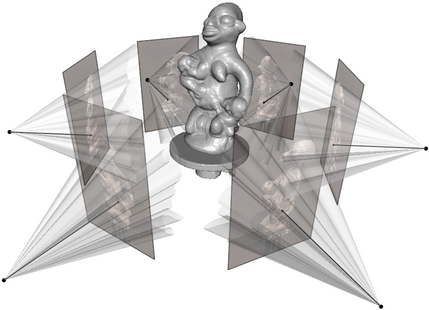
\includegraphics[width=0.2\textwidth]{images/mvs.png}} &
\raisebox{-0.75\height}{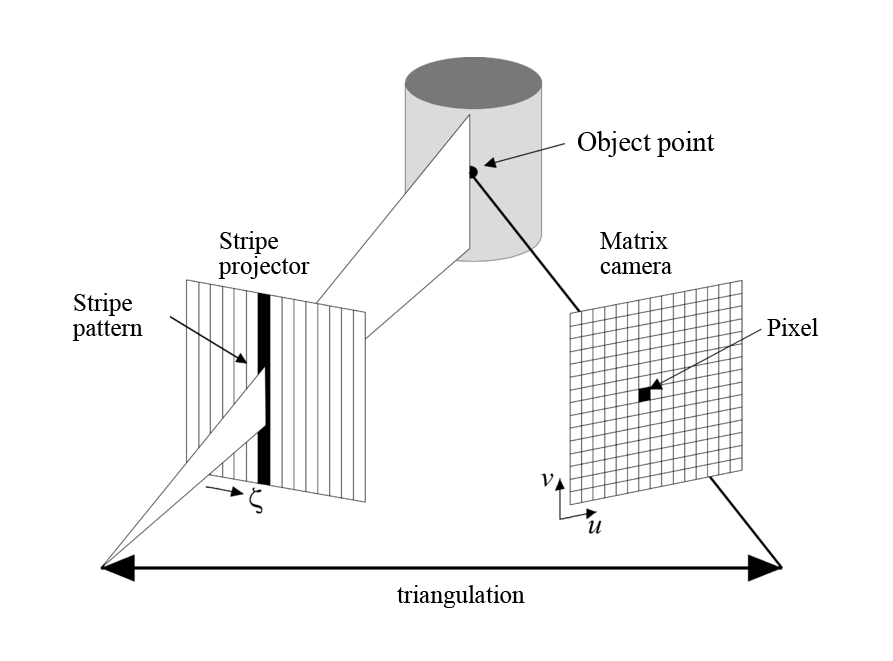
\includegraphics[width=0.2\textwidth]{images/sl.jpg}} &
Texture, Albedo, Specular \\
Shape from Intensity & 
\raisebox{-.75\height}{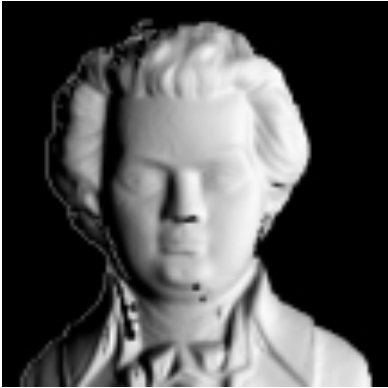
\includegraphics[width=0.15\textwidth]{images/sfs.png}} &
\raisebox{-.75\height}{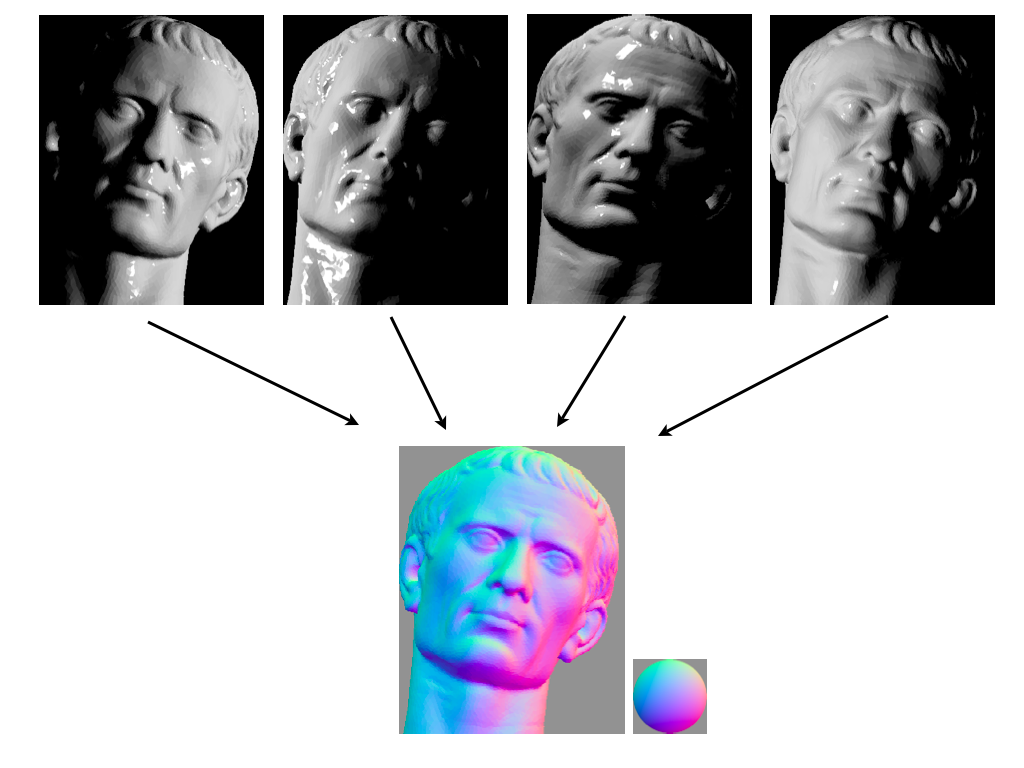
\includegraphics[width=0.2\textwidth]{images/ps.png}} &
Albedo, Specular, Geomtry \\
Shape from Silhouette &
\raisebox{-.75\height}{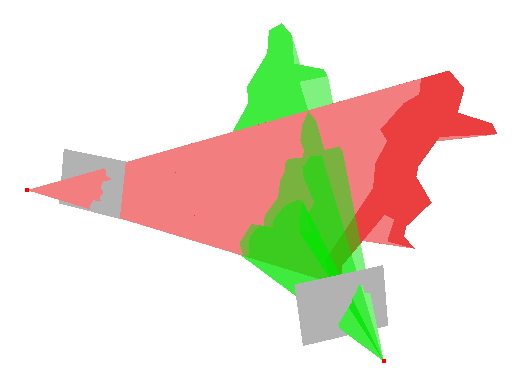
\includegraphics[width=0.2\textwidth]{images/vh.jpg}} &
\raisebox{-.75\height}{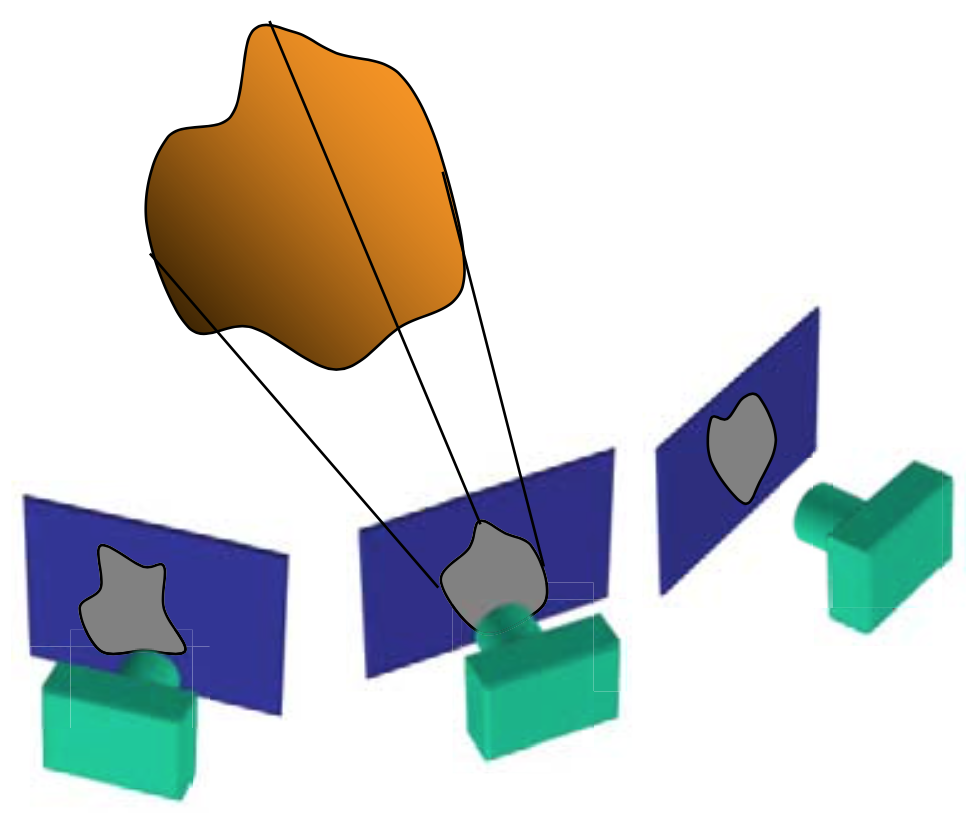
\includegraphics[width=0.2\textwidth]{images/vh_1.png}} &
Geoemtry\\
\end{tabular}
\end{figure}

\begin{alertblock}{Challenges}
1. Few algorithm works for objects with diverse range of properties;\\
2. The range of problem conditions under which an algorithm works is not known a priori.
\end{alertblock}

\end{frame}

%------------------------------------------------
\section{Development of Interface}
%------------------------------------------------
\begin{frame}{Overview of interface}

\begin{exampleblock}{3-layer interface for 3D reconstruction}
\end{exampleblock}

\begin{figure}
\centering
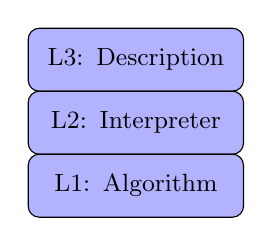
\begin{tikzpicture}[node distance=0.8cm, auto]

\node (desc) [data, font=\small] {L3: Description};
\node (interp) [data, below of=desc, font=\small] {L2: Interpreter};
\node (algo) [data, below of=interp, font=\small] {L1: Algorithm};

\end{tikzpicture}
\end{figure}

\begin{exampleblock}{Description}
  Describe visual and geometric appearance of object
\end{exampleblock}
\begin{exampleblock}{Interpreter}
  1. Translate description into an appropriate algorithm; \\
  2. Mapping: relation between problem space and algorithms.
\end{exampleblock}
\begin{exampleblock}{Algorithm}
  Underlying algorithms across varied categories.
\end{exampleblock}

\end{frame}

%------------------------------------------------
\subsection{Description of 3D Reconstruction}
%------------------------------------------------
\begin{frame}{Description: problem space}

\begin{exampleblock}{Problem space}
\end{exampleblock}
\begin{figure}
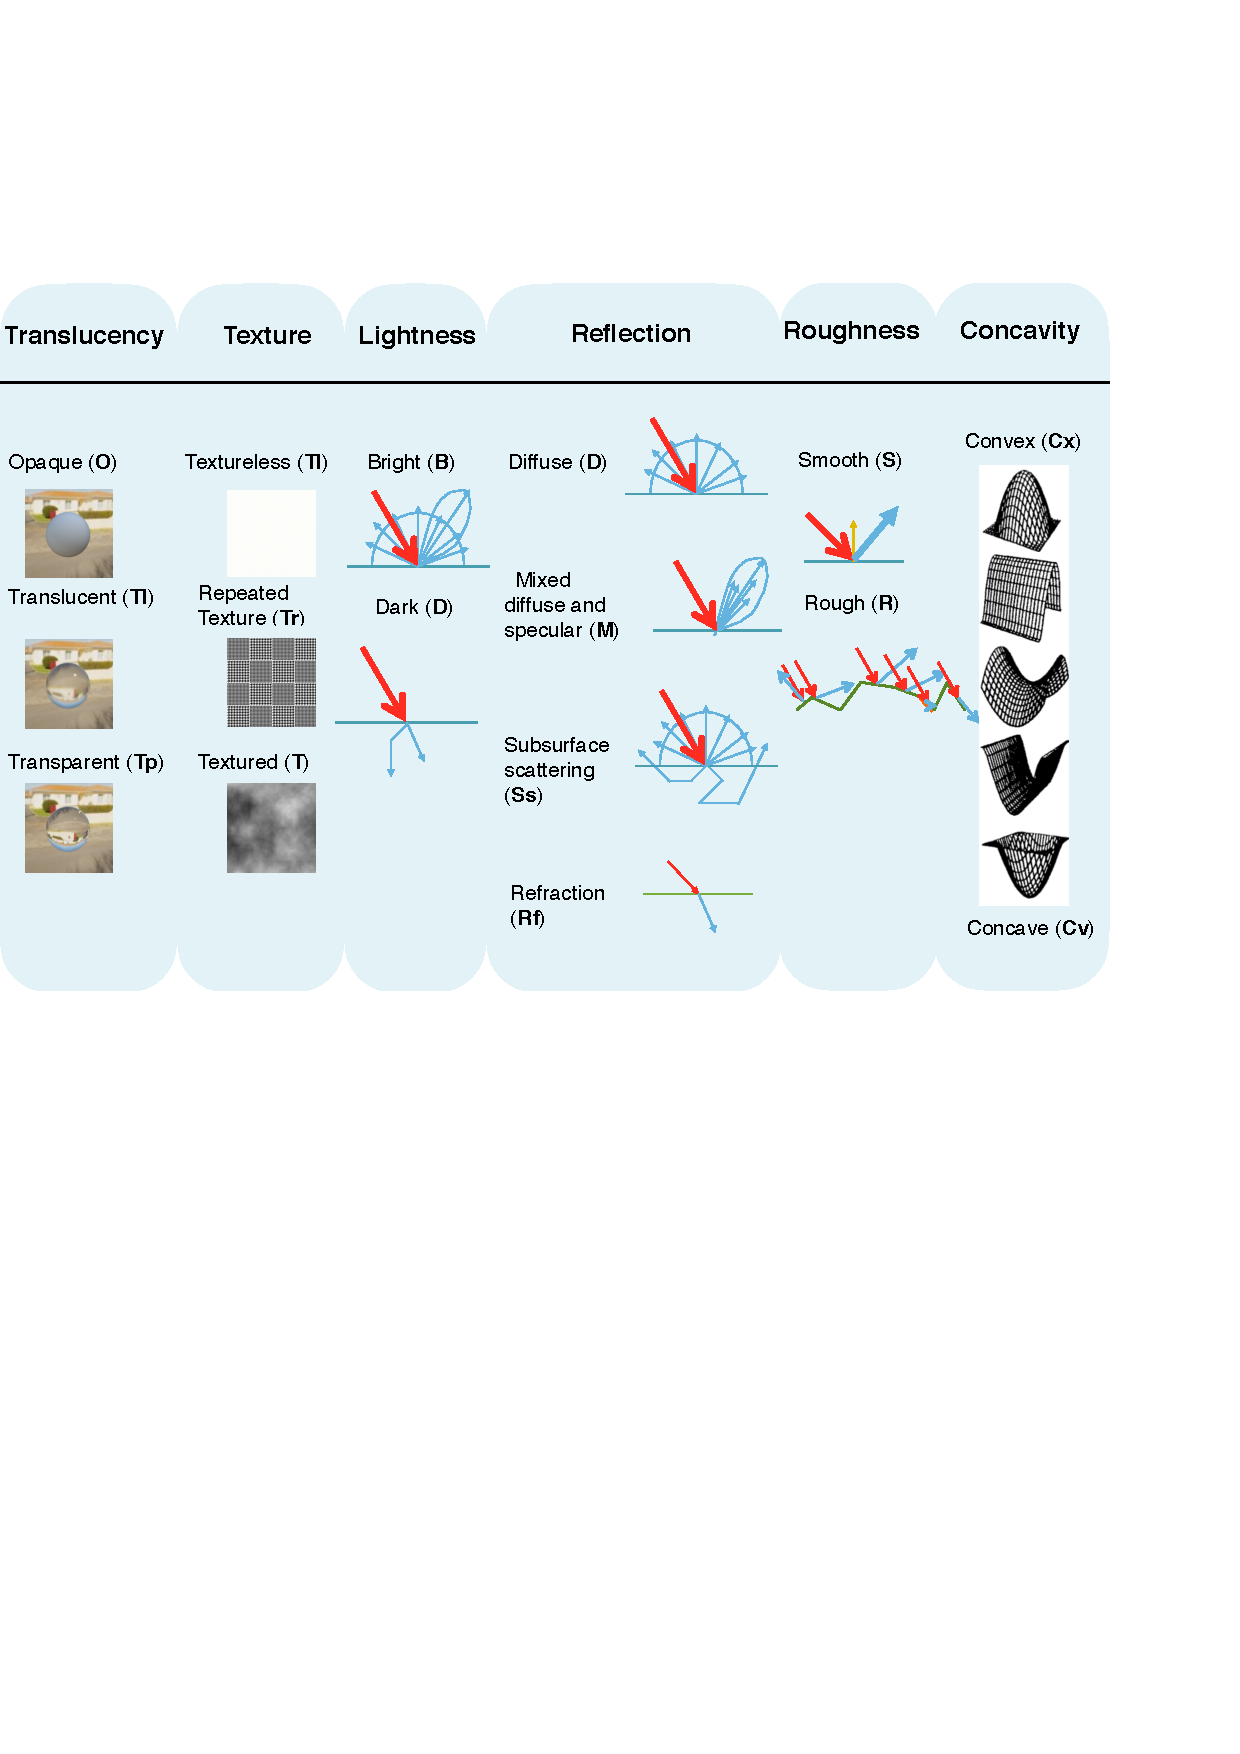
\includegraphics[width=0.55\textwidth]{prob_space/obj_class}
\end{figure}

\begin{exampleblock}{Four problem conditions}
\end{exampleblock}
\begin{figure}
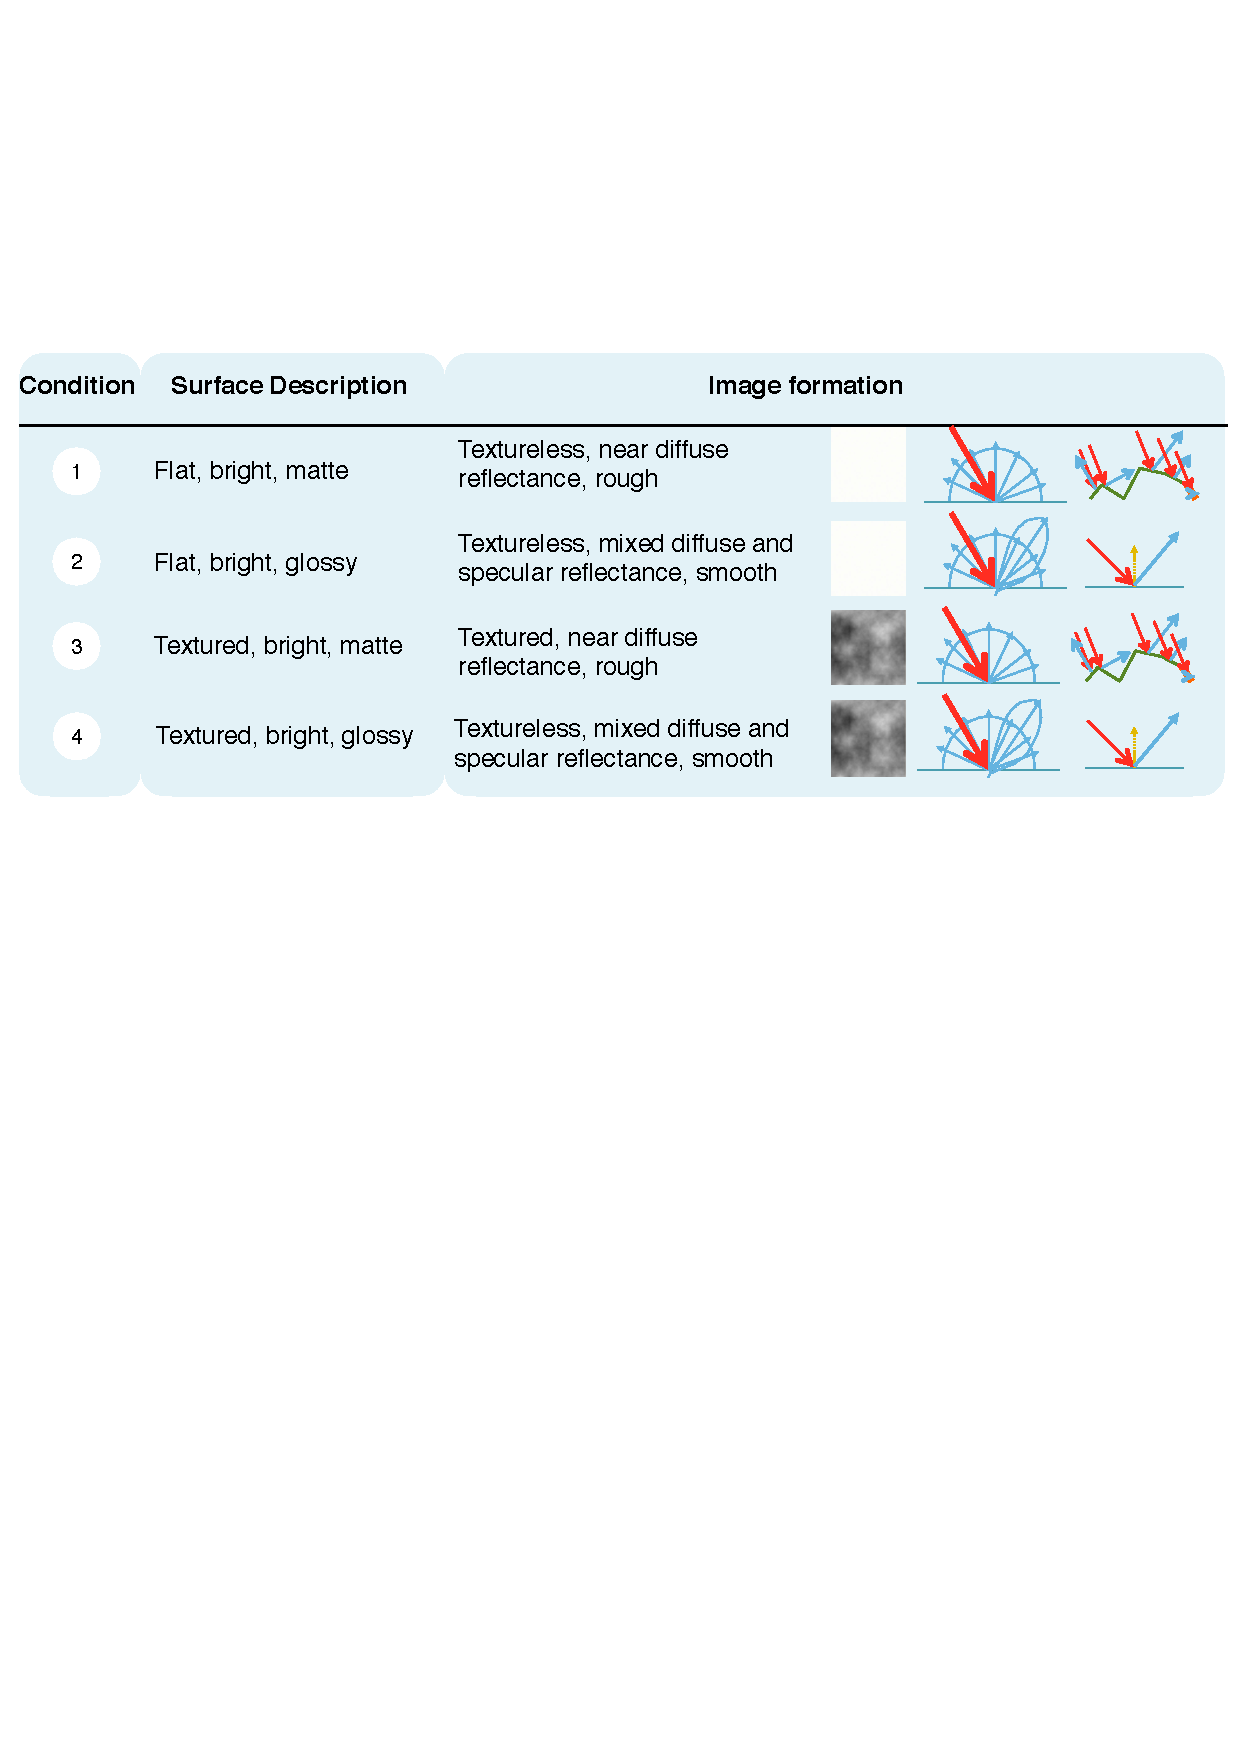
\includegraphics[width=0.55\textwidth]{prob_space/prob_cond}
\end{figure}

\begin{exampleblock}{Assumptions}

\begin{itemize}
\item \textbf{existence of algorithms}
  \begin{itemize}
  \item translucent, transparent objects need specialized methods;
  \item low surface reflectance, low reflected light.
  \end{itemize}
\item \textbf{local interaction model}
  \begin{itemize}
  \item transmission, refraction, inter-reflection;
  \item severe concavity.
  \end{itemize}
\end{itemize}

\end{exampleblock}

\end{frame}

%------------------------------------------------
\begin{frame}{Description: model and representations}

\begin{table}
  \centering
  \begin{tabular}{lp{4cm}l}
  \textbf{Model} & \textbf{Representation} & \textbf{Example}\\ \cline{1-3}
  Nature of scene & \textit{Static} \\
  Lighting & \textit{Mixed: ambient, projector, light sources} \\
  Vantage point & \textit{Medium: 10 - 50} \\
  Texture & \textit{Texture randomness} & \raisebox{-.5\height}{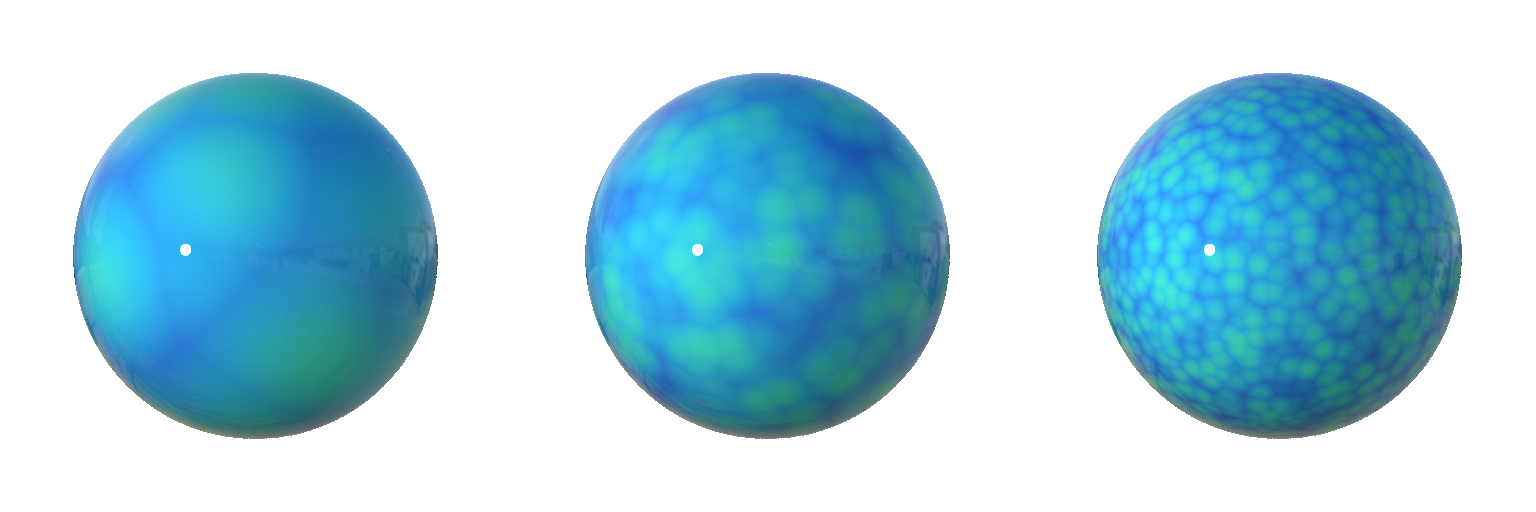
\includegraphics[width=0.3\textwidth]{mapping/setup/tex0}}\\
  Brightness & \textit{Diffuse reflectance} & \raisebox{-.5\height}{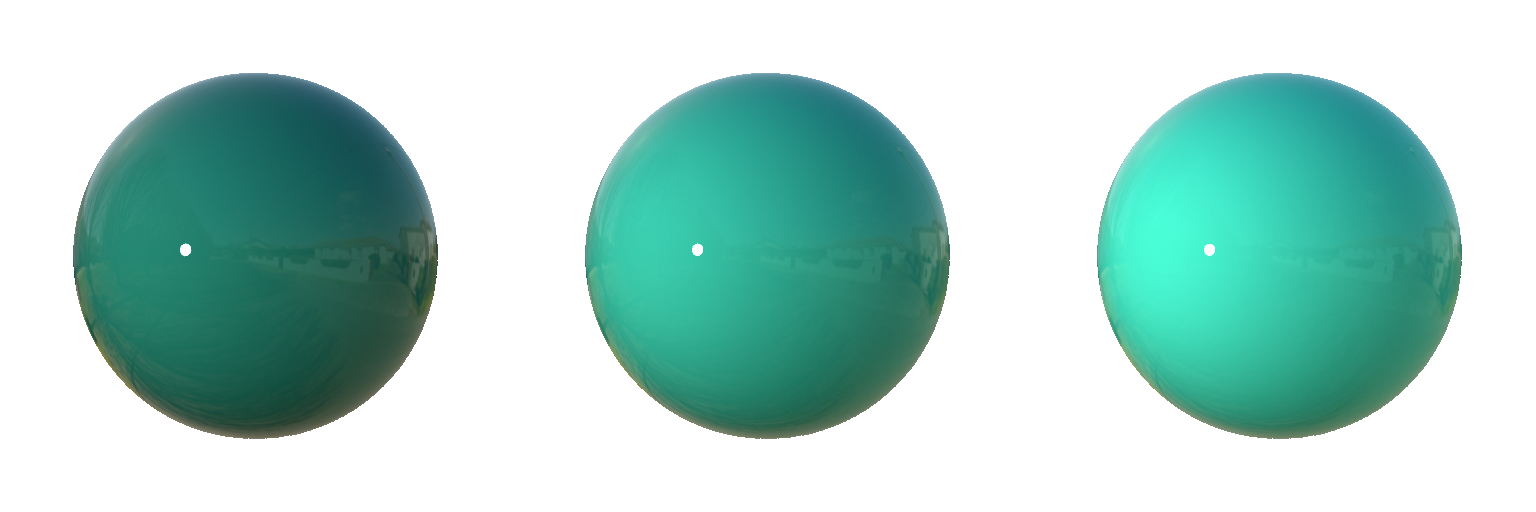
\includegraphics[width=0.3\textwidth]{mapping/setup/alb0}}\\
  Specularity & \textit{Fresnel reflectance} & \raisebox{-.5\height}{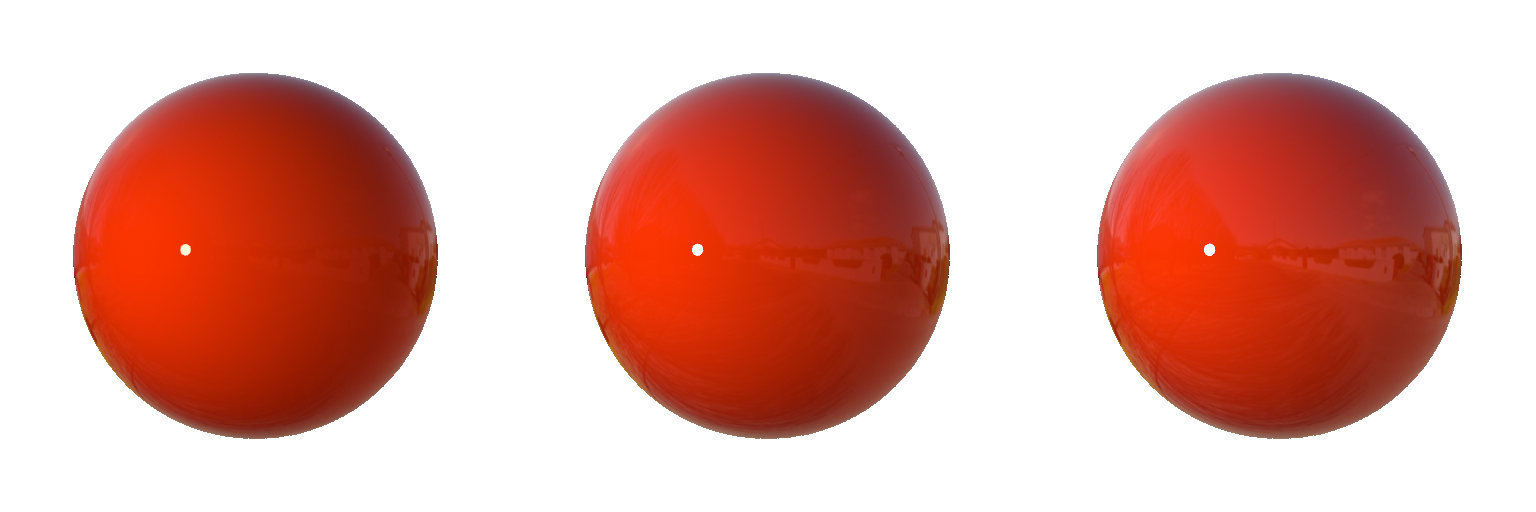
\includegraphics[width=0.3\textwidth]{mapping/setup/spec0}}\\
  Roughness & \textit{Distribution of facet normal} & \raisebox{-.5\height}{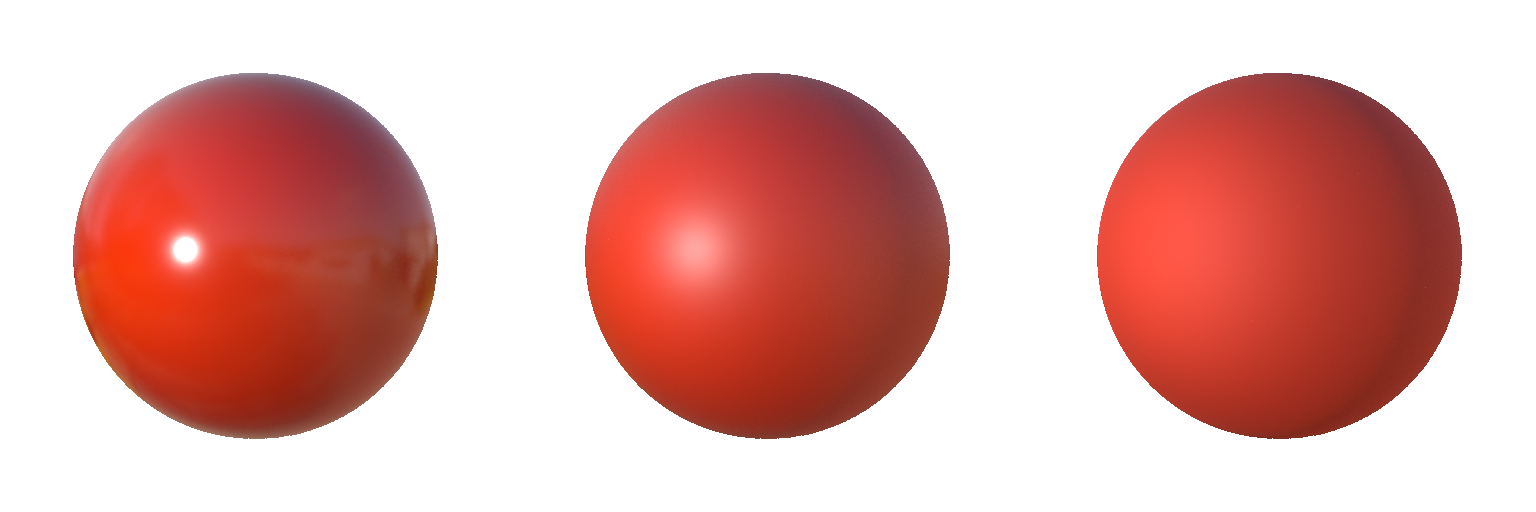
\includegraphics[width=0.3\textwidth]{mapping/setup/rough0}}\\
  % Concavity & \textit{Surface curvature}\\
  \end{tabular}
\end{table}

\end{frame}

%------------------------------------------------
\subsection{Mapping of 3D Reconstruction}
%------------------------------------------------
% \begin{frame}{Mapping: overview}

% % Investigate the problem conditions under which the algorithms can reliably work.
% \begin{figure}
% \centering
% \includegraphics[width=0.9\textwidth]{images/mapping_0.pdf}
% \end{figure}

% \end{frame}

%------------------------------------------------
\begin{frame}{Mapping: dimension reduction}

\begin{figure}
\centering
\includegraphics[width=0.8\textwidth]{images/mapping_1.pdf}
\end{figure}

Reduce problem space dimensionality by discovering properties that have an effect on algorithm performance.

\begin{figure}
\centering
\includegraphics[width=0.5\textwidth]{mapping/eval_prop/mvs_tex_spec}
\end{figure}

\end{frame}

%------------------------------------------------
\begin{frame}{Mapping: mapping construction}

\begin{figure}
\centering
\includegraphics[width=0.8\textwidth]{images/mapping_2.pdf}
\end{figure}

Discover the mapping from problem condition to algorithms.
\begin{figure}
\centering
\includegraphics[width=0.5\textwidth]{mapping/lookup_table/mvs_texture_05}
\end{figure}

\end{frame}

%------------------------------------------------
\subsection{Interpretation of 3D Reconstruction}
%------------------------------------------------
\begin{frame}{Interpreter: proof of concept}

Interpreter: selects an algorithm based on a description.

\begin{figure}[!htbp]
\centering
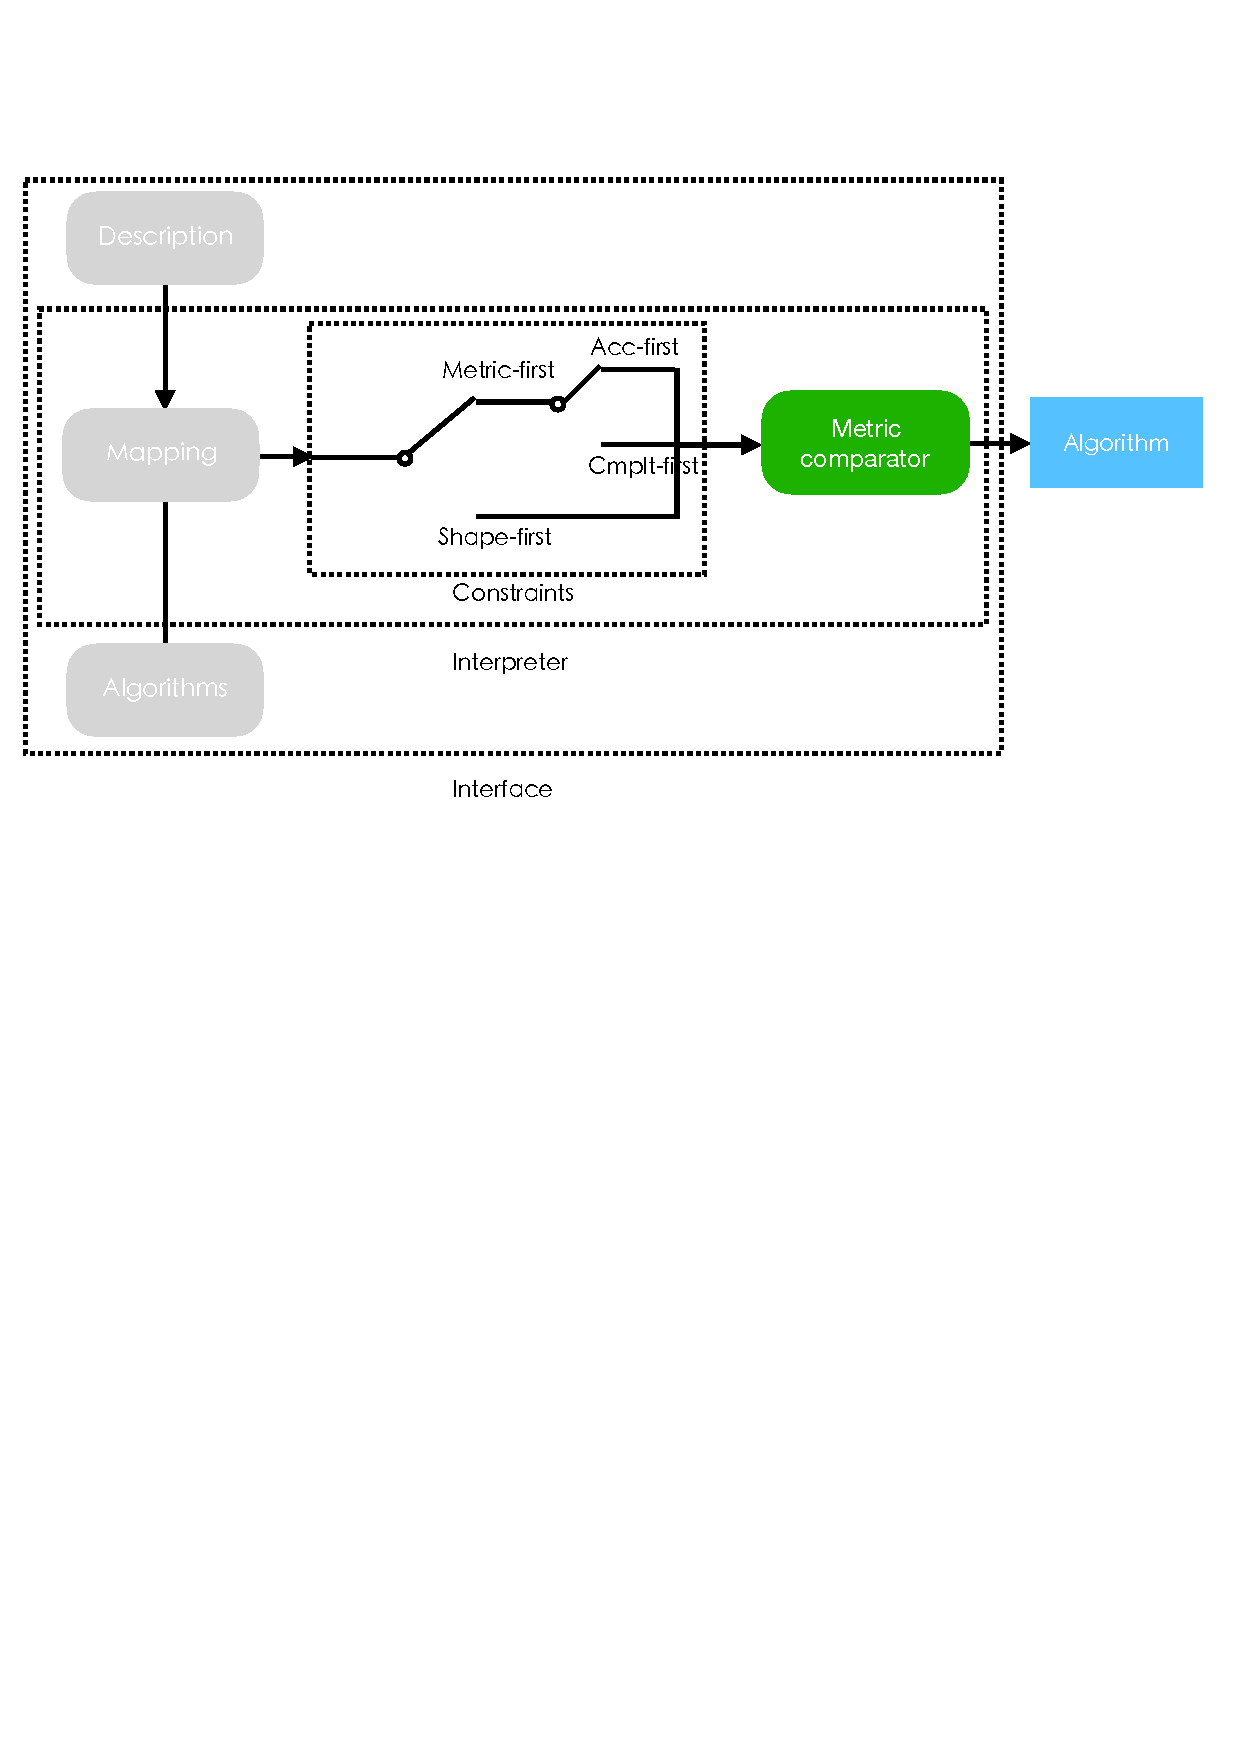
\includegraphics[width=\textwidth]{images/interpreter.pdf}
\end{figure}

\end{frame}

%------------------------------------------------
\section{Application of Interface}
%------------------------------------------------
\begin{frame}{Interpretation: evaluation questions}

\begin{exampleblock}{Evaluation questions}
\begin{enumerate}
  \item accurate description $\Rightarrow$ successful result;
  \item less accurate description $\Rightarrow$ less successful result;
  \item inaccurate description $\Rightarrow$ poor result.
\end{enumerate}
\end{exampleblock}

\begin{exampleblock}{Criteria}
  Visual comparison.
\end{exampleblock}

\begin{figure}
\centering
\begin{tabular}{ccc}
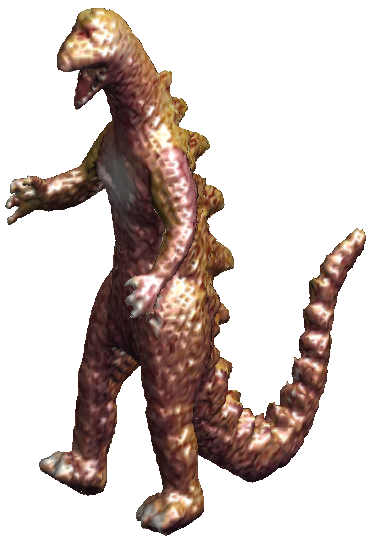
\includegraphics[width=0.2\textwidth]{images/dino.png} &
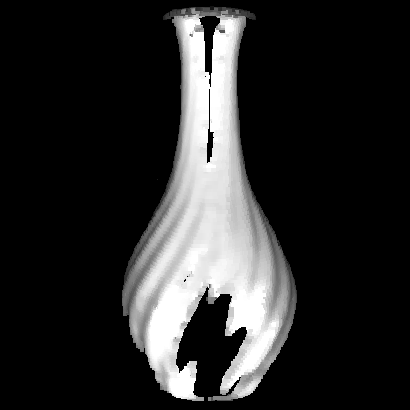
\includegraphics[width=0.2\textwidth]{interp/synth_interp/vase0_sl} &
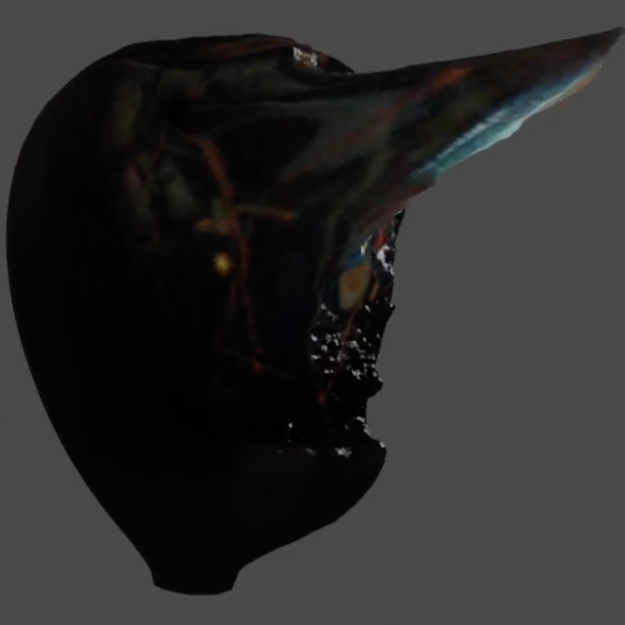
\includegraphics[width=0.2\textwidth]{interp/real_interp/vase/vase_spike} \\
accuracy & completenss & angle diff \\
\end{tabular}
\end{figure}

\end{frame}

%------------------------------------------------
\begin{frame}{Interpretation: dataset creation}

\begin{figure}
\centering
\begin{tabular}{ccc}
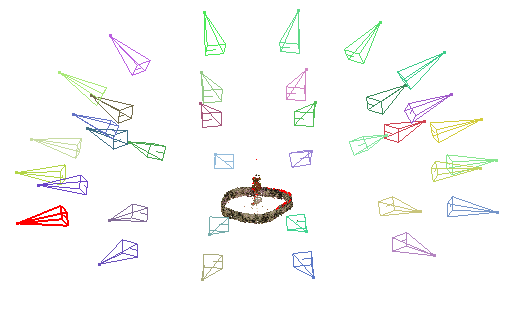
\includegraphics[width=0.3\textwidth]{images/mvs_calib.PNG} &
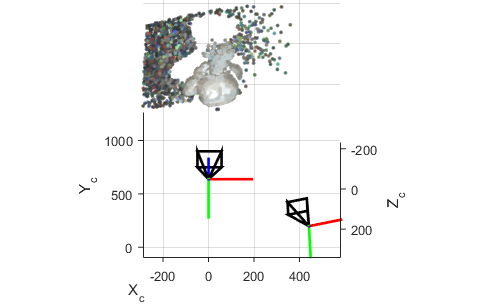
\includegraphics[width=0.3\textwidth]{images/sl_calib.png} &
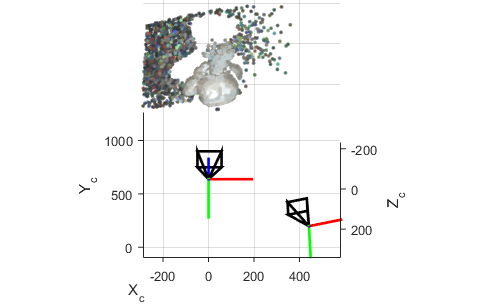
\includegraphics[width=0.3\textwidth]{images/sl_calib.png}\\
MVS\& VH & PS & SL \\
\end{tabular}
\end{figure}

\begin{table}
  \begin{tabular}{p{1cm}p{2cm}p{2.5cm}p{4cm}}
  Alg & Hardware & Config & Calibration \\
  \midrule
  MVS, VH & camera, turntable  & 3 heights, $30^\circ$ baseline angle & focal length from EXIF, extrinsics using SfM \\
  PS & camera, lamp, ref objs & random light position & no radiometric/geometric calibration performed \\
  SL & camera, projector & $10^\circ$ baseline angle & camera-projector calibration using local homography\\
  \end{tabular}
\end{table}

\end{frame}

%------------------------------------------------
\begin{frame}{Interpreter: accurate description, successful result}

\setlength{\fboxrule}{2pt}
\addtolength{\tabcolsep}{-3pt}
\begin{figure}
\centering
\begin{tabular}{ccccc}

\includegraphics[width=0.2\textwidth]{images/interp11.pdf} &
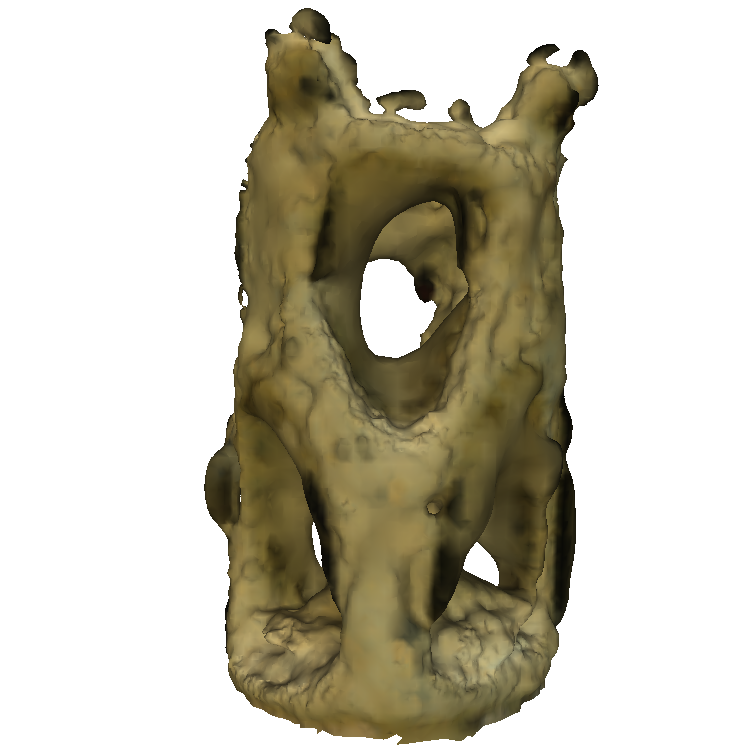
\includegraphics[width=0.15\textwidth]{interp/real_interp/statue/statue_mvs} &
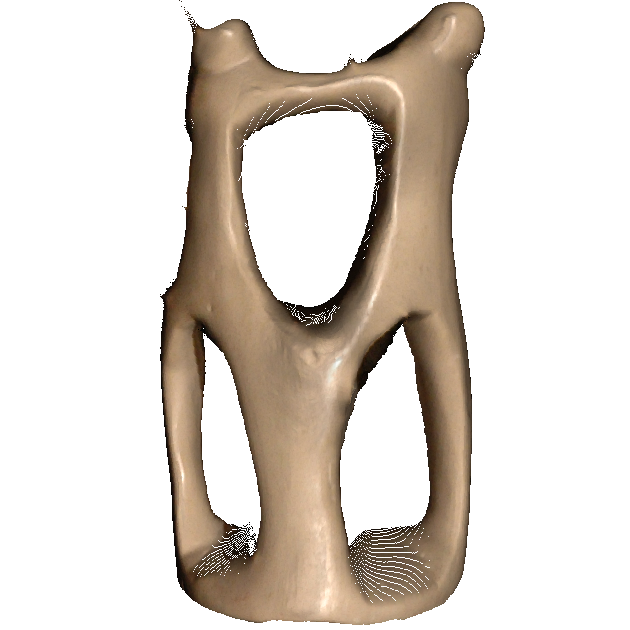
\includegraphics[width=0.15\textwidth]{interp/real_interp/statue/statue_ps} &
\fcolorbox{green}{white}{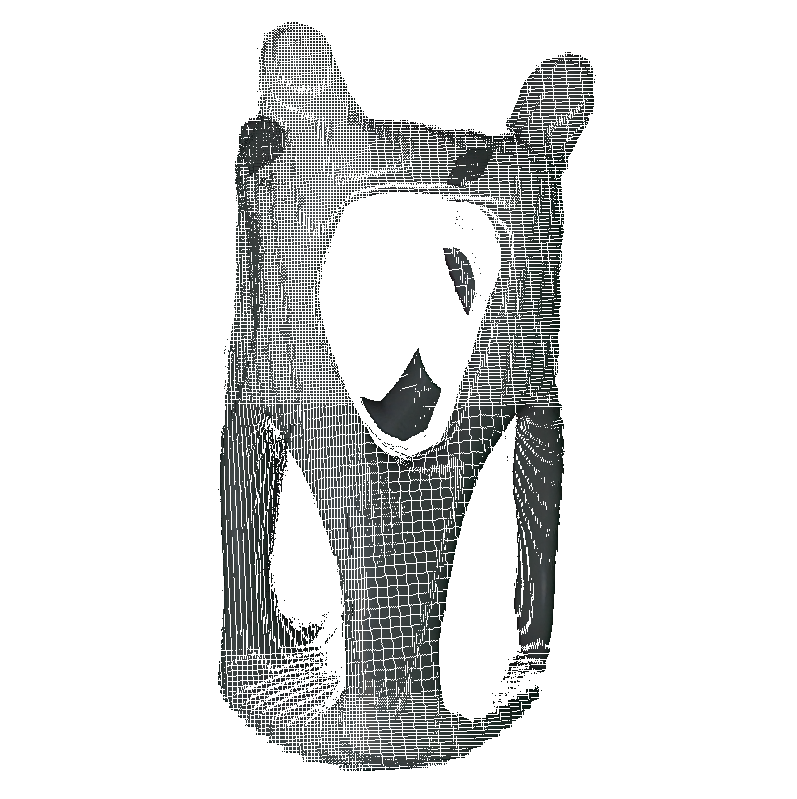
\includegraphics[width=0.15\textwidth]{interp/real_interp/statue/statue_sl}} &
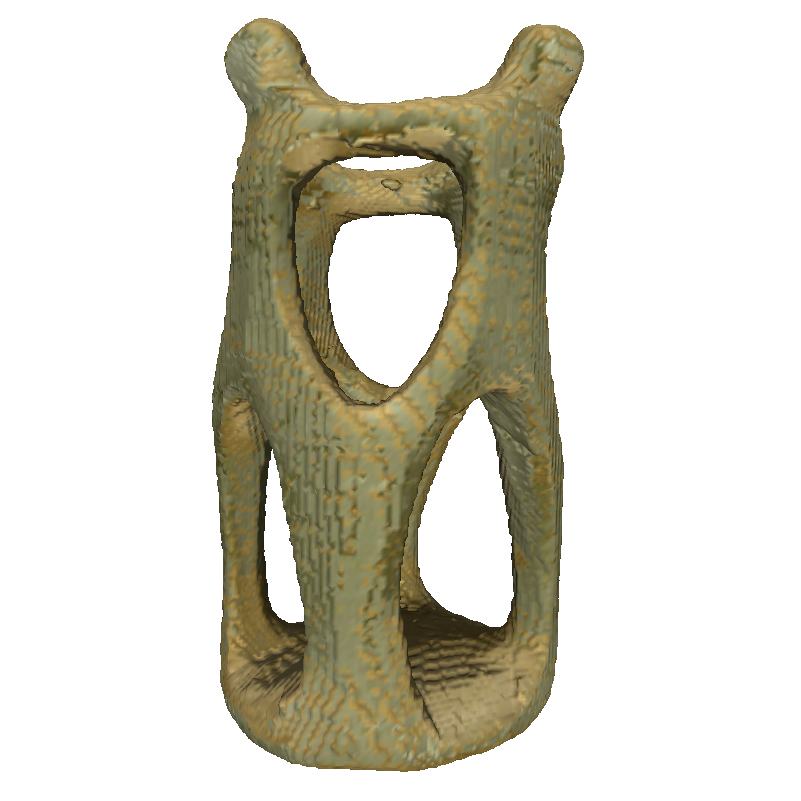
\includegraphics[width=0.15\textwidth]{interp/real_interp/statue/statue_sc} \\

% \includegraphics[width=0.2\textwidth]{images/interp21.pdf} &
% 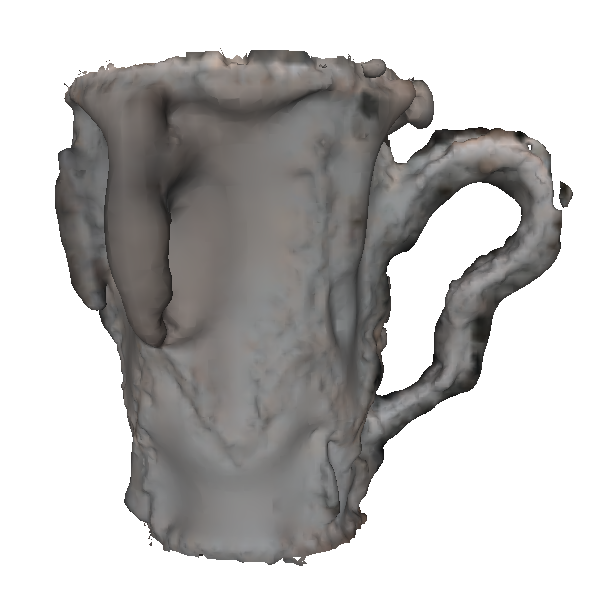
\includegraphics[width=0.15\textwidth]{interp/real_interp/cup/cup_mvs} &
% \fcolorbox{green}{white}{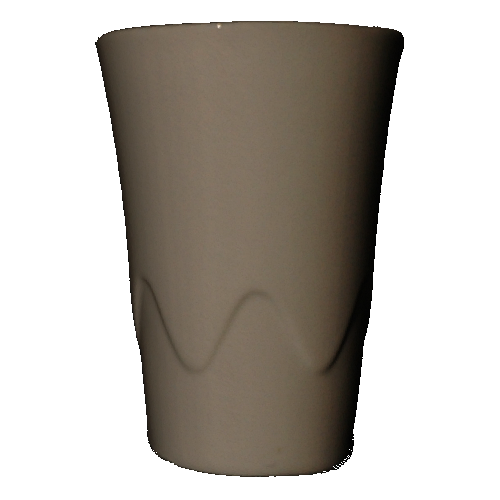
\includegraphics[width=0.15\textwidth]{interp/real_interp/cup/cup_ps}} &
% 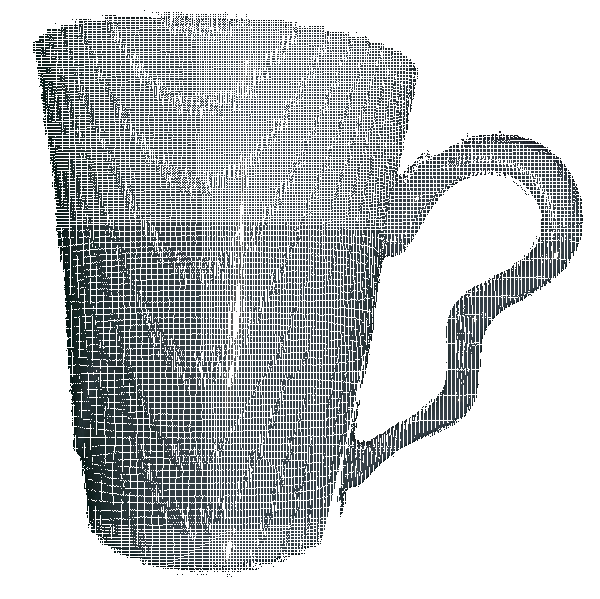
\includegraphics[width=0.15\textwidth]{interp/real_interp/cup/cup_sl} &
% 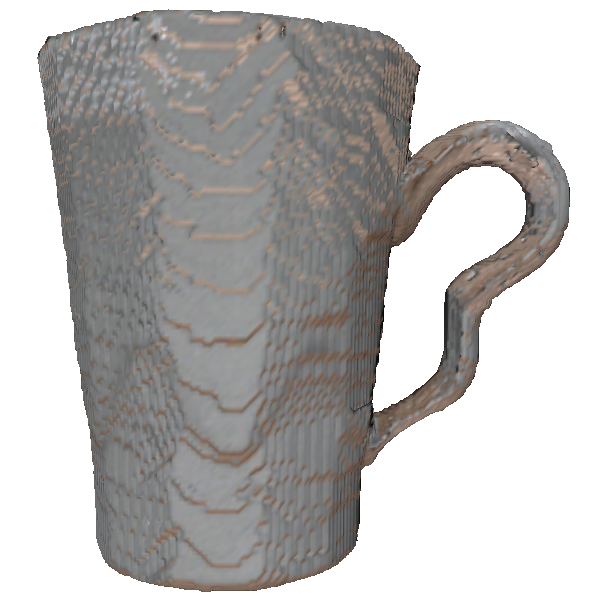
\includegraphics[width=0.15\textwidth]{interp/real_interp/cup/cup_sc} \\

% \includegraphics[width=0.2\textwidth]{images/interp31.pdf} &
% 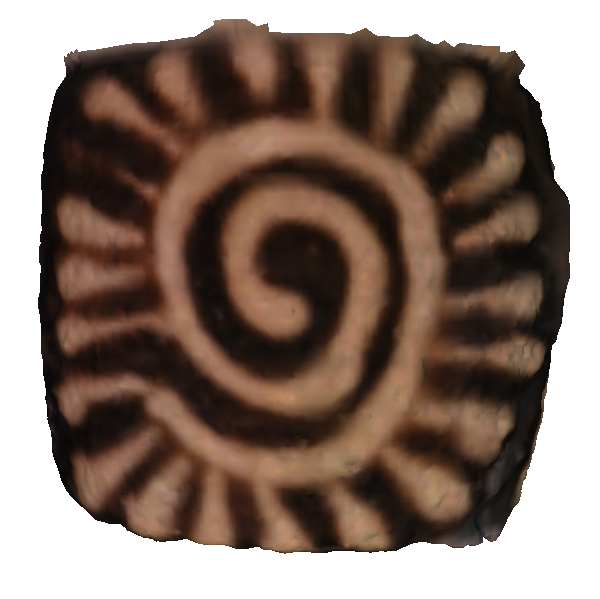
\includegraphics[width=0.15\textwidth]{interp/real_interp/pot/pot_mvs} &
% 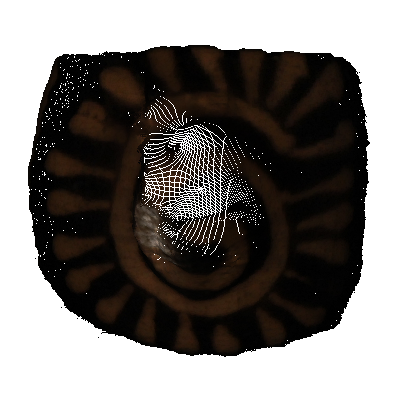
\includegraphics[width=0.15\textwidth]{interp/real_interp/pot/pot_ps} &
% \fcolorbox{green}{white}{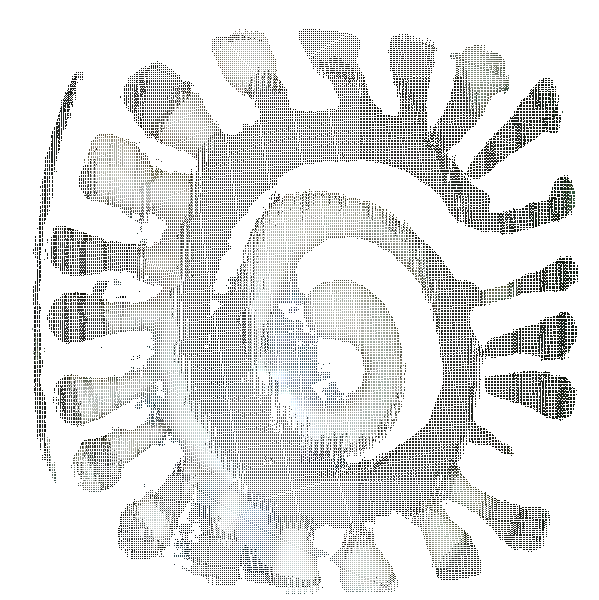
\includegraphics[width=0.15\textwidth]{interp/real_interp/pot/pot_sl}} &
% 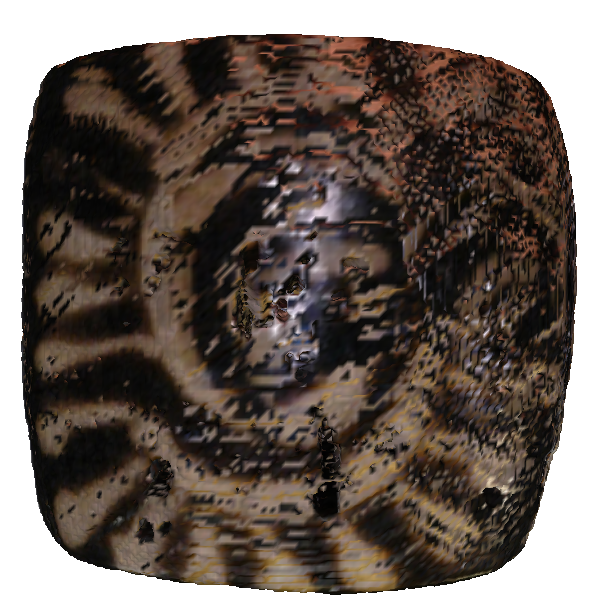
\includegraphics[width=0.15\textwidth]{interp/real_interp/pot/pot_sc} \\

\includegraphics[width=0.2\textwidth]{images/interp41.pdf} &
\fcolorbox{green}{white}{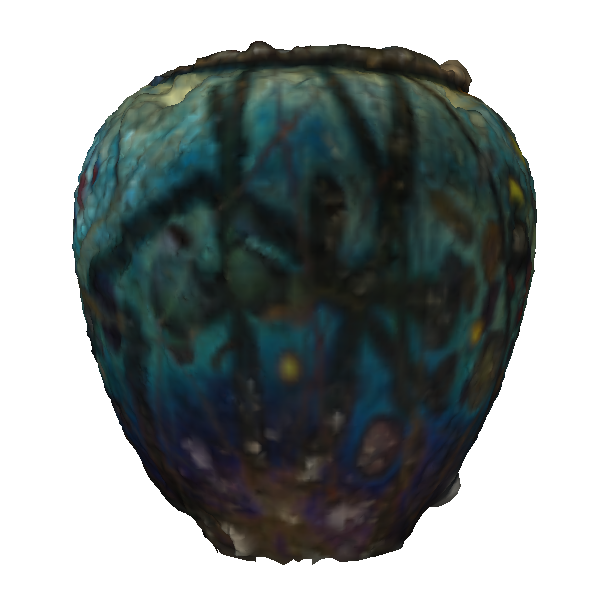
\includegraphics[width=0.15\textwidth]{interp/real_interp/vase/vase_mvs}} &
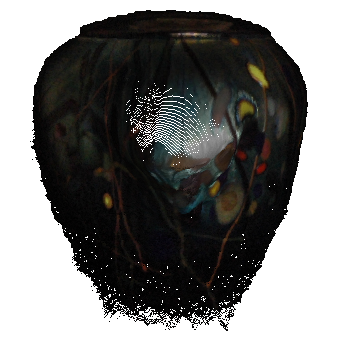
\includegraphics[width=0.15\textwidth]{interp/real_interp/vase/vase_ps} &
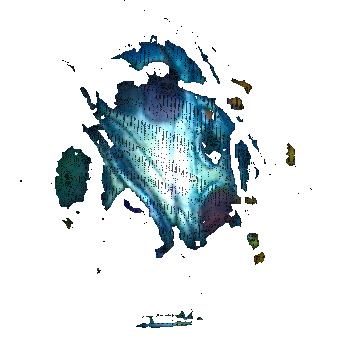
\includegraphics[width=0.15\textwidth]{interp/real_interp/vase/vase_sl} &
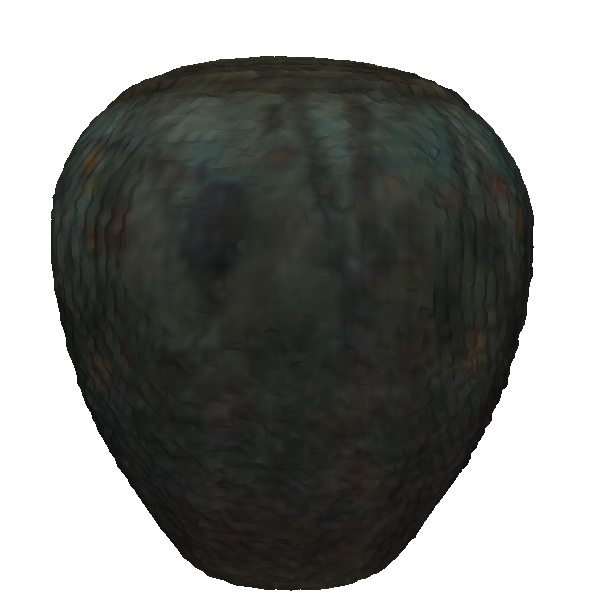
\includegraphics[width=0.15\textwidth]{interp/real_interp/vase/vase_sc} \\

\end{tabular}
\end{figure}
\addtolength{\tabcolsep}{3pt}

\begin{exampleblock}{}
\begin{itemize}
\item \textbf{Input}: correct description of problem condition;
\item \textbf{Output}: reconstruction returned by the interface is successful (one of the best) compared to the BL method.
\end{itemize}
\end{exampleblock}

\end{frame}

%------------------------------------------------
\begin{frame}{Interpreter: less accurate description, less successful result}

\setlength{\fboxrule}{2pt}
\addtolength{\tabcolsep}{-3pt}
\begin{figure}
\centering
\begin{tabular}{ccccc}

\includegraphics[width=0.2\textwidth]{images/interp12.pdf} &
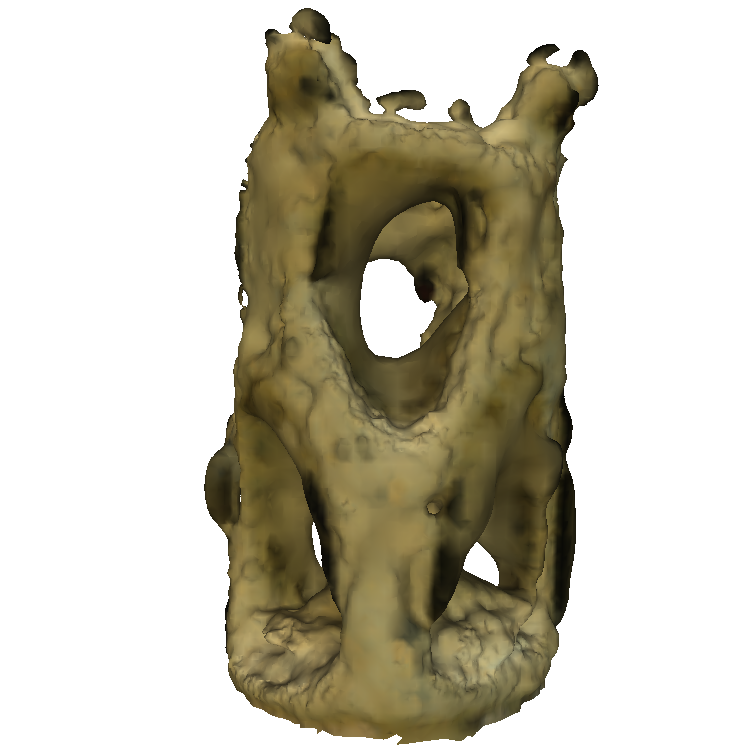
\includegraphics[width=0.15\textwidth]{interp/real_interp/statue/statue_mvs} &
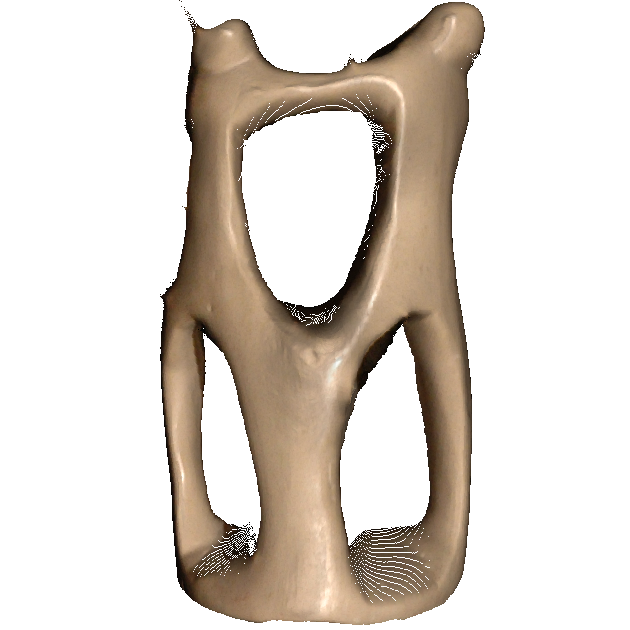
\includegraphics[width=0.15\textwidth]{interp/real_interp/statue/statue_ps} &
\fcolorbox{green}{white}{\includegraphics[width=0.15\textwidth]{interp/real_interp/statue/statue_sl}} &
\includegraphics[width=0.15\textwidth]{interp/real_interp/statue/statue_sc} \\

% \includegraphics[width=0.2\textwidth]{images/interp22.pdf} &
% \fcolorbox{red}{white}{\includegraphics[width=0.15\textwidth]{interp/real_interp/cup/cup_mvs}} &
% \fcolorbox{green}{white}{\includegraphics[width=0.15\textwidth]{interp/real_interp/cup/cup_ps}} &
% \includegraphics[width=0.15\textwidth]{interp/real_interp/cup/cup_sl} &
% \includegraphics[width=0.15\textwidth]{interp/real_interp/cup/cup_sc} \\

% \includegraphics[width=0.2\textwidth]{images/interp32.pdf} &
% \includegraphics[width=0.15\textwidth]{interp/real_interp/pot/pot_mvs} &
% \includegraphics[width=0.15\textwidth]{interp/real_interp/pot/pot_ps} &
% \fcolorbox{green}{white}{\includegraphics[width=0.15\textwidth]{interp/real_interp/pot/pot_sl}} &
% \includegraphics[width=0.15\textwidth]{interp/real_interp/pot/pot_sc} \\

\includegraphics[width=0.2\textwidth]{images/interp42.pdf} &
\fcolorbox{green}{white}{\includegraphics[width=0.15\textwidth]{interp/real_interp/vase/vase_mvs}} &
\fcolorbox{red}{white}{\includegraphics[width=0.15\textwidth]{interp/real_interp/vase/vase_ps}} &
\includegraphics[width=0.15\textwidth]{interp/real_interp/vase/vase_sl} &
\includegraphics[width=0.15\textwidth]{interp/real_interp/vase/vase_sc} \\

\end{tabular}
\end{figure}
\addtolength{\tabcolsep}{3pt}

\begin{exampleblock}{}
\begin{itemize}
\item \textbf{Input}: less correct description of problem condition, one and exactly one property is set incorrectly, which is coloured in red;
\item \textbf{Output}: reconstruction returned by the interface becomes poorer in some cases, \emph{i.e.,} the interaface selects a less successful algorithm.
\end{itemize}
\end{exampleblock}

\end{frame}

%------------------------------------------------
\begin{frame}{Interpreter: inaccurate description, poor result}

\setlength{\fboxrule}{2pt}
\addtolength{\tabcolsep}{-3pt}
\begin{figure}
\centering
\begin{tabular}{ccccc}

\includegraphics[width=0.2\textwidth]{images/interp13.pdf} &
\includegraphics[width=0.15\textwidth]{interp/real_interp/statue/statue_mvs} &
\includegraphics[width=0.15\textwidth]{interp/real_interp/statue/statue_ps} &
\fcolorbox{green}{white}{\includegraphics[width=0.15\textwidth]{interp/real_interp/statue/statue_sl}} &
\fcolorbox{red}{white}{\includegraphics[width=0.15\textwidth]{interp/real_interp/statue/statue_sc}} \\

% \includegraphics[width=0.2\textwidth]{images/interp23.pdf} &
% \fcolorbox{red}{white}{\includegraphics[width=0.15\textwidth]{interp/real_interp/cup/cup_mvs}} &
% \fcolorbox{green}{white}{\includegraphics[width=0.15\textwidth]{interp/real_interp/cup/cup_ps}} &
% \includegraphics[width=0.15\textwidth]{interp/real_interp/cup/cup_sl} &
% \includegraphics[width=0.15\textwidth]{interp/real_interp/cup/cup_sc} \\

% \includegraphics[width=0.2\textwidth]{images/interp33.pdf} &
% \includegraphics[width=0.15\textwidth]{interp/real_interp/pot/pot_mvs} &
% \includegraphics[width=0.15\textwidth]{interp/real_interp/pot/pot_ps} &
% \fcolorbox{green}{white}{\includegraphics[width=0.15\textwidth]{interp/real_interp/pot/pot_sl}} &
% \fcolorbox{red}{white}{\includegraphics[width=0.15\textwidth]{interp/real_interp/pot/pot_sc}} \\

\includegraphics[width=0.2\textwidth]{images/interp43.pdf} &
\fcolorbox{green}{white}{\includegraphics[width=0.15\textwidth]{interp/real_interp/vase/vase_mvs}} &
\fcolorbox{red}{white}{\includegraphics[width=0.15\textwidth]{interp/real_interp/vase/vase_ps}} &
\includegraphics[width=0.15\textwidth]{interp/real_interp/vase/vase_sl} &
\includegraphics[width=0.15\textwidth]{interp/real_interp/vase/vase_sc} \\

\end{tabular}
\end{figure}
\addtolength{\tabcolsep}{3pt}

\begin{exampleblock}{}
\begin{itemize}
\item \textbf{Input}: incorrect description of problem condition, all properties are set incorrectly, which are coloured in red;
\item \textbf{Output}: reconstruction returned by the interface is a poor compared to that of the BL method.
\end{itemize}
\end{exampleblock}

\end{frame}

%------------------------------------------------
\begin{frame}{Interpretation: discussions}

\begin{exampleblock}{}
\begin{itemize}
\item We have demonstrated that it is achievable to design an description-based interface so that a successful reconstruction result is obtained given a description of problem condition, without knowledge of which algorithm to use;
\item Algorithm chosen by the interpreter given a less accurate description may or may not achieve a poor result;
\item Algorithm chosen by the interpreter given inaccurate description is more likely to achieve a poorer result;
\item As the description becomes far away from the accurate one, the interpreter will select a less successful algorithm and achieve poorer result.
% \item It depends if the return algorithms has at least an overlapping with those returned if given accurate description;
% \item The reconstruction result becomes worse as the description becomes less accurate.
\end{itemize}
\end{exampleblock}

\end{frame}

%------------------------------------------------
\begin{frame}{Interpreter: summary}

\begin{figure}
\centering
\includegraphics[width=0.9\textwidth]{images/motivation1.pdf}
\end{figure}

\begin{exampleblock}{}
  \begin{itemize}
    \item \textbf{Algorithms}: description of appearance, no vision background needed, embeding new algorithms is easy;
    \item \textbf{Parameters}: property parameters are perceptually interpretable\& meaningful;
    \item \textbf{Approach}: no \textit{trial-and-error}.
  \end{itemize}
\end{exampleblock}

\end{frame}

%------------------------------------------------
\section{Conclusions}
%------------------------------------------------
\begin{frame}{Conclusions}

\begin{exampleblock}{}

\begin{itemize}
\item The proposed interface is able to produce a correct reconstruction result given an accurate description of an object;
\item The solution produced by the interface improves as the description becomes more accurate;
\item Using the description and proof of concept interpreter, we demonstrate the possibility of using descriptive properties to hide algorithm details and providing a fixed set of parameters that can be perceptually estimated.
\end{itemize}

\end{exampleblock}

\end{frame}

%------------------------------------------------
\begin{frame}{Future directions}

\begin{exampleblock}{}

\begin{itemize}
\item Develop automated approach to derive description from images;
\item Develop more advanced techniques to discover the mapping from problem conditions to algorithms;
\item Develop more sophisticated geometric model to incorporate objects with complex geometry.
\item Investigate the more precise relation between description and performance, \emph{i.e.,} if better description can lead to better performance monotonically.
% \item To deal with more complicated objects, we need more complicated properties, or ways to describe the objects, but the challenge is the easy mathematical representation might not be available.
\end{itemize}

\end{exampleblock}

\end{frame}

%------------------------------------------------
\begin{frame}[standout]

Computer vision should focus on more than \\just algorithms, but easier accessibility.

\end{frame}

\appendix
%------------------------------------------------
% Additional material
%------------------------------------------------
\begin{frame}

\begin{alertblock}{Why did you pick those objects? Is it a right dataset to validate your claim?}
\begin{itemize}
\item This objects are random, everyday objects that do NOT favour any of the selected algorithms;
\item We focus on four problem conditions and thus four representative objects. The claims are made solely for the proposed problem conditions.
\item It is challenging to get the right set of objects that meet the requirements and the capturing process is tedious for any of the methods, let alone for all of them.
\end{itemize}
\end{alertblock}

\end{frame}

%------------------------------------------------
\begin{frame}

\begin{alertblock}{How to derive parameters from description?}
\begin{itemize}
\item In current implementation, each algorithms use the ``optimal'' parameters tested on many objects;
\item The derivation of parameters from description is challenging in the sense that each algorithm has a unique set of parameters, and the relation between the description and algorithm-specific parameters is unclear.
\item This could be a future research direction, and can definitely improve the performance of the interface.
\end{itemize}
\end{alertblock}

\end{frame}

%------------------------------------------------
\begin{frame}

\begin{alertblock}{What if the number of properties is too large after dimensionality reduction?}
\begin{itemize}
\item This is definitely an issue that could happen, especially when the initial problem space is higher dimensional.
\end{itemize}
\end{alertblock}

\end{frame}

%------------------------------------------------
\begin{frame}

\begin{alertblock}{Why use the synthetic dataset?}
\begin{itemize}
\item Synthetic datasets are created under controled conditions, thus they can be used as a benchmark for the proof of concept interpreter to ensure that it actually works;
\item It is much more challenging to obtain appropriate real world datasets, thus synthetic dataset is a good alternative to gain insights into the problem.
\end{itemize}
\end{alertblock}

\end{frame}

%------------------------------------------------
\begin{frame}

\begin{alertblock}{What algorithms are chosen, why those algorithms?}

\begin{table}
\centering
\begin{tabular}{l|l}
\toprule
Technique & Summary\\
\midrule
PMVS & Patch-based, seed points propagation MVS.\\
EPS & Example-based Photometric Stereo.\\
GSL & Gray coded Structured Light technique.\\
\midrule
VH & Volumetric Visual Hull.\\
LLS-PS & Linear least squares Photometric Stereo.\\
\bottomrule
\end{tabular}
\end{table}

\begin{itemize}
\item These algorithms are the classic, and top performers among their respective class;
\item Three algorithms from three different categories are able to provide well rounded capability to the interface, which is sufficient for demonstrative purposes;
\item Additional algorithms can be easily integrated into the interface by going through the same process discussed in the thesis.
\end{itemize}
\end{alertblock}

\end{frame}

%------------------------------------------------
\begin{frame}

\begin{alertblock}{Is the problem space a bit over-simplified?}
\begin{itemize}
\item The problem space is heavily relied on the availability of existing algorithms, and the model of description. Thus properties such as translucency is omitted because they need very specialized algorithms, and many geometric properties are omitted since it is challenging to come up with semantically meaningful, and mathematic way to represent these properties;
\item This is a proof of concept demonstration that it is achievable to produce a successful reconstruction result given an accurate description, thus being comprehensive is not the priority.
\end{itemize}
\end{alertblock}

\end{frame}

%------------------------------------------------
\begin{frame}

\begin{alertblock}{The description is set manually, which is tedious and subjective, any thoughts on how to make it automated?}
\begin{itemize}
\item 
\end{itemize}
\end{alertblock}

\end{frame}

%------------------------------------------------
\begin{frame}

\begin{alertblock}{Who are the potential users, what are their applications, and how will they use the proposed interface?}
\begin{itemize}
\item Users:
\item Applications:
\item Use:
\end{itemize}
\end{alertblock}

\end{frame}

%------------------------------------------------
\begin{frame}

\begin{alertblock}{What are the next important steps?}
\begin{itemize}
\item \textbf{Description}: More sophisticated problem space and description to include objects with more complex visual and geometric properties;
\item \textbf{Mapping}: Better methods to discover the mapping from problem conditions to algorithms;
\item \textbf{Interpreter}: More sophisticated interpreter.
\end{itemize}
\end{alertblock}

\end{frame}


\end{document}
